\documentclass[10pt]{article}

\def\Type{LessonCaelan}
\def\TypeNum{Lesson 6}
\def\TypeTitle{Basic Differentiation Rules\\Key }
\def\Semester{Fall 2021} %Not Used 
\def\Course{MATH 1190 \& 1210}
\def\Targets{ {\bf\color{ForestGreen}D1}, {\bf\color{ForestGreen}D3} }

\usepackage{preambleDJ}




%%%%%%%%%%%% BEGIN DOCUMENT %%%%%%%%%%%%%%%
%%%%%%%%%%%% BEGIN DOCUMENT %%%%%%%%%%%%%%%
%%%%%%%%%%%% BEGIN DOCUMENT %%%%%%%%%%%%%%%
%%%%%%%%%%%% BEGIN DOCUMENT %%%%%%%%%%%%%%%
%%%%%%%%%%%% BEGIN DOCUMENT %%%%%%%%%%%%%%%



\begin{document}

\pagestyle{otherpages}
\thispagestyle{firstpage}
\vs{.5}

\textbf{Intended Learning Outcomes}
After this lesson, you will be able to 

\begin{itemize}
    \item Take the derivative using the power rule. (\target{D3})
    \item Take the derivative of a constant. (\target{D3})
    \item Take the derivative of $e^x$ (\target{D3})
    \item Take the derivative using the sum, difference, and constant multiple rules. (\target{D3})
    \item Apply algebraic simplification before taking the derivative using the power rule. (\target{D3})
    \item Describe the relationship between the derivative and slope of the tangent line.(\target{D1})
\end{itemize}

\vspace{-0.5cm}

\hrulefill
\paragraph*{GOAL:} The goal of this activity is to learn to use the basic rules of differentiation to find derivatives of power functions, and to solve some problems in which derivatives are needed.\\

{\bf\color{blue} Warm-up Exercise 1.} Certain radical or fraction expressions can be rewritten as outputs of power functions. For example, if $a$, $b$, and $n$ are nonzero, then:\\

\,\hfill $x^{a/b} = \sqrt[b]{x^a}$ \hfill $x^{-n} = \dfrac{1}{x^n}$ \hfill\,\\

Rewrite the following powers of $x$ as radical and/or fraction expressions.
\tasksA{4}{
\task $x^{3/5} =\blue{ \sqrt[5]{x^3} }$
\task $x^{5/3} =\blue{ \sqrt[3]{x^5} }$
\task $x^{-4} =\blue{\dfrac{1}{x^4}} $
\task $x^{-5/3}=\blue{\dfrac{1}{\sqrt[3]{x^5}}}$
}
\vs{.5}
%\begin{align*}
%(a) & \,x^{3/5} = \hspace{1in} && (b) \,x^{5/3} = \hspace{1in} && (c) \,x^{-4} = \hspace{1in} && (d) \,x^{-5/3} = \hspace{1in}\\[0.1in]
%\end{align*}

Re-write the following as a power of $x$.
\tasksAR{3}{
\task  $\sqrt[3]{x^4} =\blue{x^{4/3}}$
\task $\sqrt[4]{x^3} =\blue{x^{3/4}}$
\task $\sqrt{x} = \blue{x^{1/2}}$
\vs{.5}
\task $\dfrac{1}{x^2} = \blue{x^{-2}}$
\task $\dfrac{3}{x^2} = \blue{3x^{-2}}$
\task $\dfrac{1}{\sqrt[3]{x^4}} = \blue{\dfrac{1}{x^{4/3}}=x^{-4/3}}$
}
%\begin{align*}
%(d) & \,\sqrt[3]{x^4} = \hspace{1in} && (e) \,\sqrt[4]{x^3} = \hspace{1in} && (f) \,\sqrt{x} = \hspace{1in}\\[0.5in]
%(g) & \,\frac{1}{x^2} = \hspace{1in} && (h) \,\dfrac{3}{x^2} = \hspace{1in} && (i) \,\dfrac{1}{\sqrt[3]{x^4}} = \hspace{1in} \\[0.1in]
%\end{align*}

\hs{.5}

{\bf \color{blue} Warm-up Exercise 2.} Review some of the important differentiation rules from the class prep activity by filling them in here:
\tasksA{3}{
\task $\ds \frac{d}{dx} \left[x^n\right] =\blue{nx^{n-1}} $
\task $\ds \frac{d}{dx}[c] = \blue{0}$
\task $\ds \frac{d}{dx} [cf(x)] =\blue{c \frac{d}{dx} [f(x)]=c \,f^{\prime}(x)}$ 
\vs{.25}
\task $\ds \frac{d}{dx} \left[f(x) - g(x) \right] = $
\blue{
\al{
\frac{d}{dx} [f(x)] - \frac{d}{dx}[g(x)]  &=\hs{.5}\\
f^{\prime}(x)-g^{\prime}(x)&\\
}
}
\task $\ds \frac{d}{dx} [f(x) + g(x)] =$
\blue{
\al{
\frac{d}{dx} [f(x)] + \frac{d}{dx}[g(x)]  &=\hs{.5}\\
f^{\prime}(x)+g^{\prime}(x)&\\
}
}
\task  $\ds \frac{d}{dx} [e^x] = \blue{e^x}$
}
%%%%%%%%%
\newpage%
%%%%%%%%%

{\exercise{\color{ForestGreen}D3}} Practice using the rules on the first page by finding the following derivatives:\\

\def\sz{1.1}
\tasksA{2}{
\task $\dfrac{d}{dx}\Big[ x^{4} \Big]=\blue{4x^3}$
\task $\dfrac{d}{dx}\Big[ x^{-3} \Big] =\blue{-3x^{-3-1}=-3x^{-4}}$
\vs{.5}
\task $\dfrac{d}{dx}\Big[ -7 \Big]=\blue{0}$
\task $\dfrac{d}{dx}\Big[ x^{-2/5} \Big]=\blue{-\dfrac{2}{5}x^{-2/5-1}=-\dfrac{2}{5}x^{-2/5-5/5} =-\dfrac{2}{5}x^{-7/5} }$
\vs{.5}
\task $\dfrac{d}{dx}\Big[ 2x^5 \Big]=\blue{2\cdot 5x^4=10x^4}$ 
 \task  $\dfrac{d}{dx}\left[ \dfrac37 \right]=\blue{0}$
 \vs{.5}
 \task  $\dfrac{d}{dx}\left[3e^x\right]=\blue{3\cdot e^x=3e^x}$
 \task $\dfrac{d}{dx}\left[\dfrac{1}{\sqrt[3]{x^4}}\right]=\blue{\dfrac{d}{dx}[x^{-4/3}]=-\dfrac{4}{3}x^{-4/3-1}=-\dfrac{4}{3}x^{-7/3}}$
 \vs{.5}
\task  $\dfrac{d}{dx}\left[ \dfrac{3}{x^2} \right]=\blue{\dfrac{d}{dx}[3x^{-2}]=3\cdot -2x^{-3}=-6x^{-3}}$
\task $\dfrac{d}{dx}\left[2x^5-\dfrac{3}{x^2}+3e^x+\dfrac1{\sqrt[3]{x^4}}-\dfrac37\right]=\blue{}$
\blue{
\al{
\dfrac{d}{dx}\left[2x^5 \right]-\dfrac{d}{dx}\left[\frac{3}{x^2} \right]+\dfrac{d}{dx}\left[3e^x \right]+\dfrac{d}{dx}\left[\dfrac{1}{\sqrt[3]{x^4}} \right]-\dfrac{d}{dx}\left[\dfrac{3}{7}\right]&\\
=10x^4+6x^{-3}+3e^x-\frac{4}{3}[x^{-7/3}-0&
\intertext{(see earlier work in this problem)}
}
}
%\vs{\sz}
\task $\dfrac{d}{dx} \left[\dfrac{x^3+5x^2-1}{\sqrt[3]{x}}\right]=$ \vs{-.5}
\blue{
\al{
\hs{1.3}&\dfrac{d}{dx} \left[\dfrac{x^3+5x^2-1}{x^{1/3}}\right]\\
=&\dfrac{d}{dx}\left[\dfrac{x^3}{x^{1/3}} \right]+\dfrac{d}{dx}\left[\dfrac{5x^2}{x^{1/3}} \right]-\dfrac{d}{dx}\left[\dfrac{1}{x^{1/3}} \right] \\
=&\ds \dfrac{d}{dx}\left[x^{8/3} \right]+\dfrac{d}{dx}\left[ 5x^{5/3}\right]-\dfrac{d}{dx}\left[x^{-1/3} \right]\\
=&\ds \frac{8}{3}x^{5/3}+\frac{25}{3}x^{2/3}+\frac{1}{3}x^{-4/3}
}
}
}

%%%%%%%%%
\newpage%
%%%%%%%%%

{\exercise{\color{ForestGreen}D1}} Are there any points on the graph of $\ds f(x) = \frac{1}{3}x^3 - \frac{5}{2}x^2 + 5x - 11 $ at which the tangent line to the graph has a slope of $-1$? If so, then find all such points. If not, then explain why. 
\sol{
$f^{\prime}(x)$ is slope of tangent line at $x$.  So we assume $f^{\prime}(x)=-1$ and solve for $x$.

\al{
f^{\prime}(x)&=-1\\
\frac{1}{3}\cdot 3x^{3-1}-\frac{5}{2}\cdot 2x^{2-1} =5-0&=-1\\
x^2-5x+5&=-1\\
x^2-5x+6&=0\\
(x-3)(x-2)&=0
}

Thus $x=3$ or $x=2$. \\
 When $x=3$, $\ds y=f(3)=-\frac{19}{2}$. \\
 When $x=2$, $\ds f(2)=-\frac{25}{3}.$
Points on graph where slope is$-1$ occur at $\ds \left( 3, -\frac{19}{2}\right)$ and at $\ds \left( 2, -\frac{25}{3}\right)$.
}
\vs{.5}

In the next exercise, we'll introduce an important object in calculus: the {\bf linearization} of a function. In addition to creating the foundation for many topics in applied \& higher mathematics, linearizations help connect the big ideas of calculus.

\begin{minipage}[t][3in][t]{0.45\textwidth}
{\bf\color{blue}Extra Practice 1.} The graph of $f(x)=\sqrt{x}$ is depicted to the right.
\begin{enumerate}
\item[i.] Find an equation $y=L(x)$ of the tangent line to the graph at the point $(4,2)$. This function $L$ is called the {\bf linearization} of $f$ at $4$. Sketch the graph of the linearization (i.e. tangent line) to the right.
\sol{
We have a point, $(4,2)$ and need a slope to find the equation of the tangent line.  Since $f^{\prime}{x}$ is slope of tangent line and $f(x)=\sqrt{x}=x^{1/2}$, we find $\ds f^{\prime}(x)=\frac{1}{2}^{-1/2}=\frac{1}{2x^{1/2}}=\frac{1}{\sqrt{x}}$.  $\ds m=f^{\prime}(4)=\frac{1}{2 \sqrt{4}}=\frac{1}{4}$. Equation of tangent line is $$L(x)=m(x-a)+b=\frac{1}{4}(x-4)+2=\frac{1}{4}x+1$$
}
\end{enumerate}
\end{minipage}
%
\hfill
%
\begin{minipage}[t][3in][t]{0.45\textwidth}
\,\begin{center}
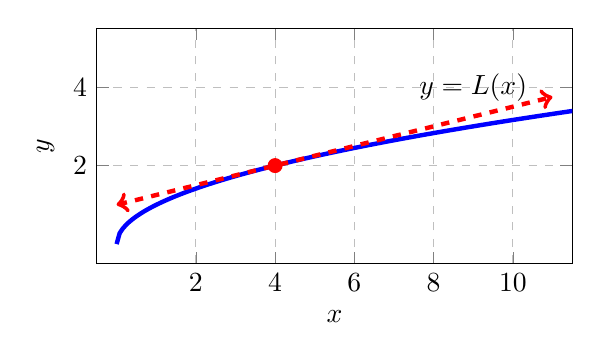
\begin{tikzpicture}[scale=1]
  \begin{axis}[
%    axis y line = left,
%    axis x line = bottom,
    xtick       = {2,4,6,8,10},
    xticklabels = {$2$,$4$,$6$,$8$,$10$},
    xlabel      = {$x$},
    ytick       = {2,4},
    yticklabels = {$2$,$4$},
    ylabel      = {$y$},
    samples     = 160,
    domain      = 0:12,
    restrict y to domain=-10:100,
    xmin = -0.5, xmax = 11.5,
    ymin = -0.5, ymax = 5.5,
    grid=both, grid style=dashed,
    width=3in, height=1.8in
  ]
  %
  %\addplot[blue, ultra thick, mark=none, smooth] coordinates{ (0,1) (0.5,1.25) (1,1) (1.5,0.75) (2,1) (2.5,1.5) (3,3)};
  \addplot[blue, ultra thick, mark=none] {x^(1/2)};
    \addplot[red, dashed, ultra thick, domain =0:11, <->] {1/4*(x-4)+2};
      \node at (9,4) {\red{$y=L(x)$}};
     \filldraw[red] (4,2) circle (2.5pt);
  %\addplot[name path=g, domain=-1:3.5, black, thick, mark=none, ] {0.5*e^x};
  %
\end{axis}
\end{tikzpicture}
\end{center}
\end{minipage}

%
%\hfill\,

\begin{enumerate}
\item[ii.] Calculate $f(4.1)$ using a calculator and $L(4.1)$ by hand. What do you notice about these two quantities? How does the picture above also reflect your observation? Explain.\\
\mpageT{.5}{.5}{
\sol{
From a calculator $f(4.1)=2.0248...$. Using our linearization, $L(4.1)=\frac{1}{4}\cdot 4.1+1=2.025$ This is very close! It suggests that $f(x)\approx L(x)$. If we zoom in on our graph, we can that $L(x)$, the red dashed line, is virtually indistinguishable from $f(x)$ for values of $x$ close to $4.1$. \\\\
In general, the {\em linearization} $L(x)$ of a function $f(x)$ at a given value  $x=a$ is a decent approximation for values of $x$ close to $a$.
}
}{
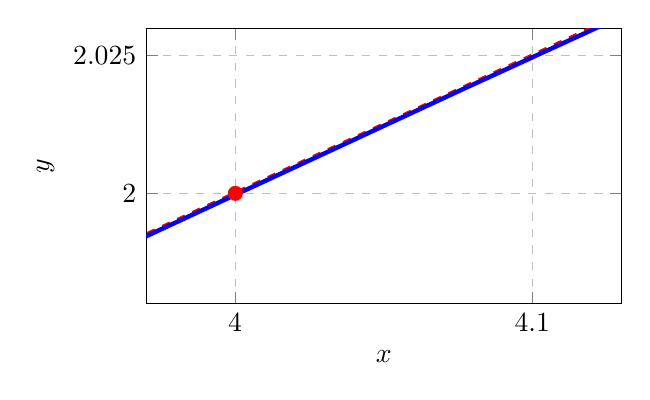
\begin{tikzpicture}[scale=1]
  \begin{axis}[
%    axis y line = left,
%    axis x line = bottom,
    xtick       = {2,4,4.1, 6,8,10},
    xticklabels = {$2$,$4$,$4.1$,$6$,$8$,$10$},
    xlabel      = {$x$},
    ytick       = {2,2.025,4},
    yticklabels = {$2$,$2.025$,$4$},
    ylabel      = {$y$},
    samples     = 160,
    domain      = 0:12,
    restrict y to domain=-10:100,
    xmin = 3.97, xmax = 4.13,
    ymin = 1.98, ymax = 2.03,
    grid=both, grid style=dashed,
    width=3in, height=2in
  ]
  %
  %\addplot[blue, ultra thick, mark=none, smooth] coordinates{ (0,1) (0.5,1.25) (1,1) (1.5,0.75) (2,1) (2.5,1.5) (3,3)};
    \addplot[red, dashed, ultra thick, domain =0:11, <->] {1/4*(x-4)+2};
    \addplot[blue, ultra thick, mark=none] {x^(1/2)};
      \node at (9,4) {\red{$y=L(x)$}};
     \filldraw[red] (4,2) circle (2.5pt);
  %\addplot[name path=g, domain=-1:3.5, black, thick, mark=none, ] {0.5*e^x};
  %
\end{axis}
\end{tikzpicture}
}
\vfill

%\item[iii.] Looking at the graph above, how do you expect the output values $L(x)$ and $f(x)$ to be related in general? For which input values $x$ do you think your hypothesized relationship will be valid? Explain your thoughts and observations in words and/or mathematics.

%\vfill

\end{enumerate}

%\vfill

%%%%%%%%%
\newpage%
%%%%%%%%%
\paragraph*{PREVIEW:} This problem previews a major topic in calculus: building mathematical models and using calculus to optimize them.\\ 

{\bf\color{blue}Extra Practice 2.}\reversemarginpar\marginnote{\fbox{\bf\color{RedOrange}A3}} {A book designer decided that the pages of a book should have $1$-in. margins at the top and bottom and $1/2$ in. margins on the sides. She further stipulated that each page should have an area of $50$ in$^2$.  }

%\graphicsL{PrintedPageP}{6.5}
\mpageTth{.25}{.5}{.3}{
\graphicsC{printedPage}{1.5}
}{
The labeling in the figure to the left and the restriction that $xy=50$ allows us to express the area $f$ of the printed region (in square inches) as a function of page width(in inches): $$f(x)=52-2x-\frac{50}{x}, \qquad1<x<25$$
}{
%\graphicsR{pageGraph}{1.75}
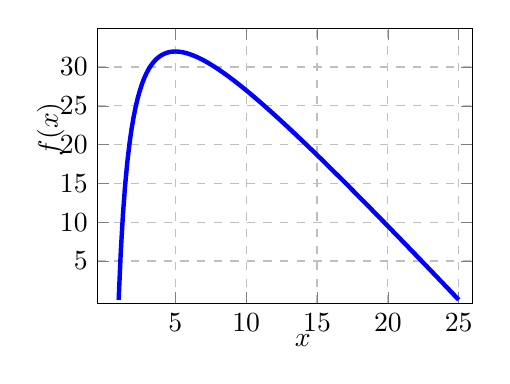
\begin{tikzpicture}[scale=1]
  \begin{axis}[
%    axis y line = left,
%    axis x line = bottom,
    xtick       = {5,10,15,20,25},
    xticklabels = {$5$,$10$,$15$,$20$,$25$},
    xlabel      =$x$,
    x label style={anchor=west},
    ytick       = {5,10,15,20,25,30},
   % yticklabels = {},
    ylabel      = {$f(x)$},
    y label style={anchor=west},
    samples     = 160,
    domain      = 0:12,
    restrict y to domain=-10:100,
    xmin = -0.5, xmax = 26,
    ymin = -0.5, ymax = 35,
    grid=both, grid style=dashed,
    width=2.5in, height=2in
  ]
  %
  %\addplot[blue, ultra thick, mark=none, smooth] coordinates{ (0,1) (0.5,1.25) (1,1) (1.5,0.75) (2,1) (2.5,1.5) (3,3)};
  \addplot[blue, ultra thick, domain=1:25, mark=none] {52-2*x-50/x};
  %\addplot[name path=g, domain=-1:3.5, black, thick, mark=none, ] {0.5*e^x};
  %
\end{axis}
\end{tikzpicture}
}
\vs{-.2}
\enumA{
\item  Using the plot of $f$ provided, above right,  what value of $x$ appears to maximize the area of the printed region? Call this value $x_0$.
\sol{It appears that $x_0\approx 5$ maximizes the graph on the right.}
{\large
$$x_0=\,\unline{.5}{\blue{$5$}}{.25}$$
}

\item Let $x_0$ be the number you identified in (a).  Based on the graph, what seems to be  the value of $f'(x_0)$? 
\sol{The tangent line appears flat which means slope is $f^{\prime}(5)=0$}
{\large
$$f'(x_0)=\,\unline{.5}{\blue{$0$}}{.25}$$
}

\item Find $f'(x)$. \sol{
\al{
 f(x)&=52-2x-\frac{50}{x}=52-2x-50x^{-1}\\
f^{\prime}(x)&=-2-50( -1x^{-2})=-2+\frac{50}{x^2}
}
}


\item Use your answer for $f'$ to the previous part to confirm your guess in part (b) is correct.  

\sol{
$$f^{\prime}(5)=-2+\frac{50}{5^2}=-2+\frac{50}{25}=-2+2=0$$
}

}

\end{document}
